\documentclass[a4paper,11pt]{article}
\pdfoutput=1 % if your are submitting a pdflatex (i.e. if you have
             % images in pdf, png or jpg format)

\usepackage{jinstpub} % for details on the use of the package, please
                      % see the JINST-author-manual

\usepackage{lineno}
\usepackage{url}
\usepackage{hyperref}

\newcommand{\vtrxp}{VTRx+}
\newcommand{\mrad}{Mrad}
\newcommand{\fig}{Figure}

% \linenumbers

\title{Development of a high bandwidth readout chain for the CMS Phase-2 pixel upgrade}

%% %simple case: multiple authors, same institution
\author{C. Smith}
\affiliation{The University of Kansas,\\Lawrence, Kansas 66045, USA}

% e-mail addresses: only for the corresponding author
\emailAdd{caleb.smith@ku.edu}

\abstract{
The CMS collaboration is building a new inner tracking pixel detector for the High-Luminosity LHC.
Each pixel readout chip will be controlled with a single serial input stream at 160 Mbps and will send out data via four current mode logic (CML) 1.28 Gbps outputs.
The readout chips will be grouped in modules and connected with up to 1.6 m long low-mass electrical links to Low-Power Gigabit Transceivers (lpGBT) and Versatile Link PLUS Transceiver (\vtrxp) modules that send the data optically to off-detector electronics at 10 Gbps.
The development and the characterization of these components is presented along with system tests of the readout chain.
}

% \keywords{Only keywords from JINST's keywords list please}
% See JINST keywords here: https://jinst.sissa.it/jinst/help/keywordsList.jsp

\keywords{Front-end electronics for detector readout, optical detector readout concepts, radiation-hard electronics}

% \arxivnumber{1234.56789} % only if you have one

\collaboration[c]{on behalf of the CMS tracker collaboration}

% if you write for a special issue this may be useful
\proceeding{Topical Workshop on Electronics for Particle Physics\\
  September 20--24, 2021\\
  Online event}

\begin{document}
\maketitle
\flushbottom

% Comment on abbreviations
% We suggest not to abbreviate: ``section'', ``appendix'', ``figure''
% and ``table'', but ``eq.'' and ``ref.'' are welcome. Also, please do
% not use \texttt{\textbackslash emph} or \texttt{\textbackslash it} for
% latin abbreviaitons: i.e., et al., e.g., vs., etc.

\section{Introduction}
\label{sec:introduction}

% The High-Luminosity LHC (HL-LHC)~\cite{ref:hllhc} will provide CMS experiment~\cite{ref:cms} with a peak instantaneous luminosity of $7.5 \times 10^{34} \mathrm{cm}^{-2} \mathrm{s}^{-1}$.
% Compared to the LHC, the HL-LHC will have up to 200 proton-proton collisions (pileup) per event and will result in a higher radiation fluence.
% To prepare for this data taking environment, the CMS Tracker will be fully replaced in the Phase-2 upgrade~\cite{ref:tdr,ref:orfanelli}.

In preparation for the High-Luminosity LHC (HL-LHC)~\cite{ref:hllhc}, the CMS Tracker will be fully replaced in the Phase-2 upgrade~\cite{ref:cms,ref:tdr,ref:orfanelli}.
The new inner tracker will have about two billion silicon pixels installed,
and hybrid pixel modules will process sensor data using a custom readout chip initially developed by the RD53 collaboration~\cite{ref:rd53}.
% The detector will be built using hybrid pixel modules that process sensor data using a custom readout chip initially developed by the RD53 collaboration~\cite{ref:rd53}.
Each readout chip on the detector needs a control link to receive trigger, clock, commands, and settings from off-detector electronics as well as data links to send pixel data to off-detector electronics.
The high bandwidth control and data links are split into two stages: electrical links and optical links.
System tests of these electrical and optical links are presented.

\section{Data Readout Chain}
\label{sec:readout}

An overview of the data readout chain for the inner tracker is shown in \fig~\ref{fig:readout}.
High bandwidth electrical and optical links are used to establish control and data links between pixel modules on the CMS detector and Data Trigger Control (DTC) boards in the counting room.
Low-mass electronic links (e-links) up to 1.6 meters long provide 160 Mbps control links (downlinks) and 1.28 Gbps data links (uplinks) between pixel modules and portcards.
Optical fibers connect portcards, which are mounted on the support structure inside the detector, to DTC boards in the counting room to establish 2.5 Gbps control links (downlinks) and 10 Gbps data links (uplinks).
The portcards each carry three Low-Power Gigabit Transceivers (lpGBT)~\cite{ref:lpgbt_1} and three Versatile Link PLUS Transceiver (\vtrxp) modules~\cite{ref:vtrxp}.
The lpGBTs convert optical signals to electrical signals (and vice versa), and the \vtrxp\space modules establish optical links with the DTC boards.

\begin{figure}[htbp]
\centering
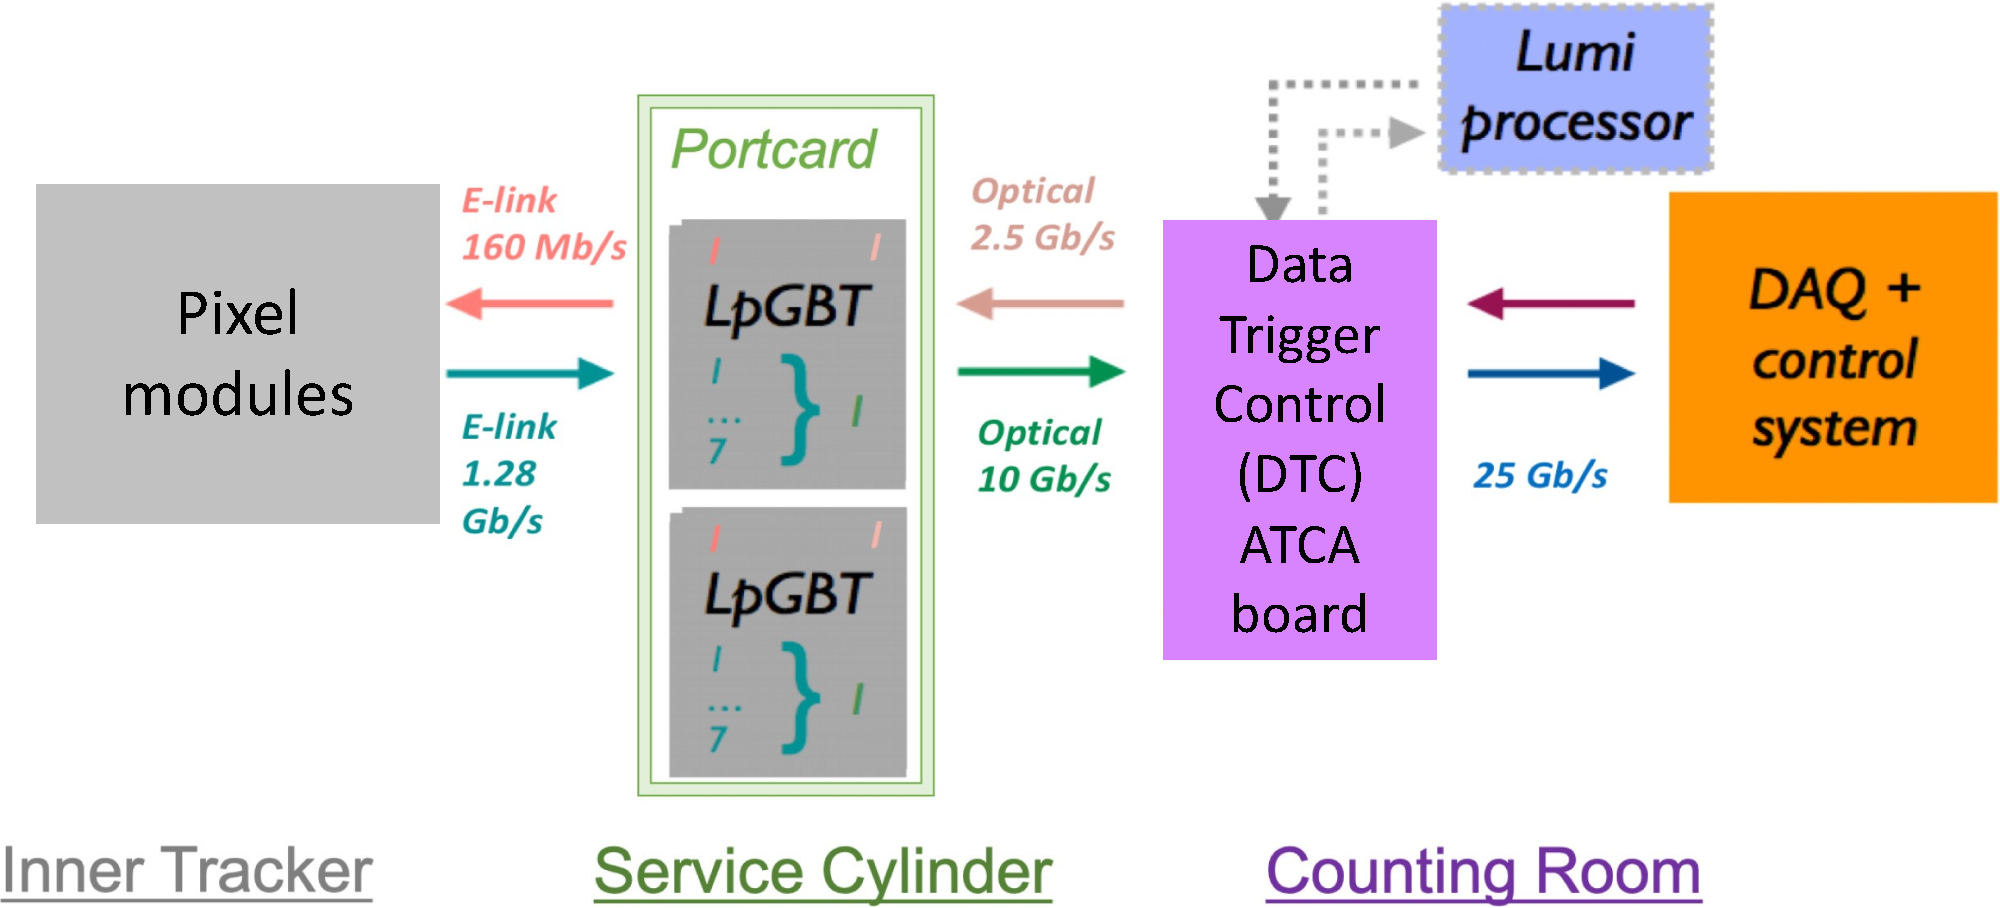
\includegraphics[width=0.70\textwidth,origin=c]{../figures/IT_System_Readout_2-crop.pdf}
\caption{
\label{fig:readout}
System readout architecture for the inner tracker~\cite{ref:orfanelli}. Pixel modules communicate with portcards through e-links. Portcards communicate with Data Trigger Control (DTC) boards through optical links.
}
\end{figure}

\section{Electrical Links}
\label{sec:electrical}

% =============
% E-link design
% =============

The electrical links (e-links) are created using low mass, small diameter twisted pair cables.
One end of a twisted pair electrical link is shown in \fig~\ref{fig:elink}.
E-link bundles are made to connect to modules and provide each module with one control link twisted pair and multiple data link twisted pairs.
Each twisted pair is produced using two 36 American Wire Gauge (AWG) copper core (127 microns in diameter) wires surrounded by polyimide insulation (45 microns thick) that are twisted together with 4 twists per inch.
The pairs are soldered to small, 20 micron thick PCBs that can plug into Molex connectors with 300 micron pitch~\cite{ref:molex45}.
To improve durability and handling, the soldered wires are secured with a non-conductive epoxy, and then the bundle is lashed together using polyimide braiding.

\begin{figure}[htbp]
\centering
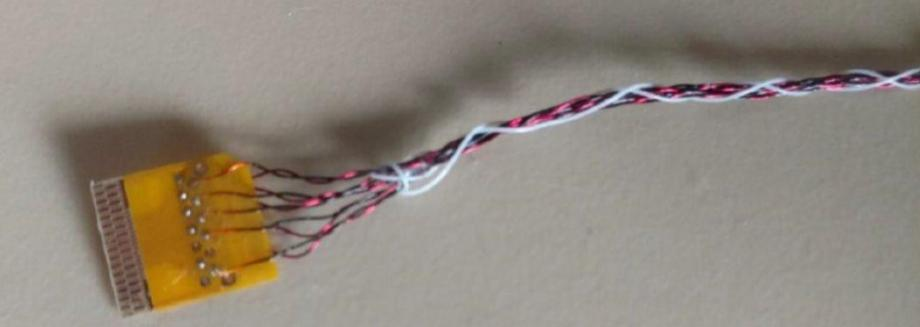
\includegraphics[width=0.4\textwidth,origin=c]{../figures/e-link-1.jpg}
\caption{
\label{fig:elink}
One end of a twisted pair electrical link (e-link).
}
\end{figure}

% ==============
% E-link testing
% ==============

Prototype low-mass electrical links are developed and characterized with a series of measurements.
The signal quality is assessed using eye diagrams, which overlay transitions between binary states from repeated measurements of the signal over a time interval.
% The eye diagram amplitude and jitter are used to quantify the quality of the differential signal and identify any distortion.
Bit error rate scans are used to characterize signal integrity across e-links.
Cross talk effects from channels within an e-link bundle (internal) and from multiple bundles (external) are studied.

% ==================
% E-link performance
% ==================

In one system test of the e-links, an RD53 chip on a Single Chip Card (SCC) is read out over e-links using an FC7 mezzanine card~\cite{ref:fc7}, as shown in \fig~\ref{fig:tap0_vs_length}.
E-links of two gauges (34 and 36 AWG) and different lengths (from 0.35 to 2.0 meters) are used in the readout chain.
Bit error rates are determined using a pseudorandom binary sequence (PRBS) that is sent from the RD53 chip to the FC7 mezzanine card.
The amplitude of the PRBS signal is varied using the ``TAP0'' pre-emphasis digital-to-analog converter (DAC) setting, which controls the amplitude of the signal output by the current mode logic (CML) driver on the RD53 chip.
For this test, the amplitude is increased until the bit error rate of $10^{-11}$ is reached.
Longer e-links require a larger signal amplitude to maintain a given bit error rate.
Good performance is seen for e-links up to 2.0 meters.

\begin{figure}[htbp]
\centering
\includegraphics[width=0.50\textwidth,origin=c]{../figures/fc7_elink_scc_setup.jpg}
\qquad
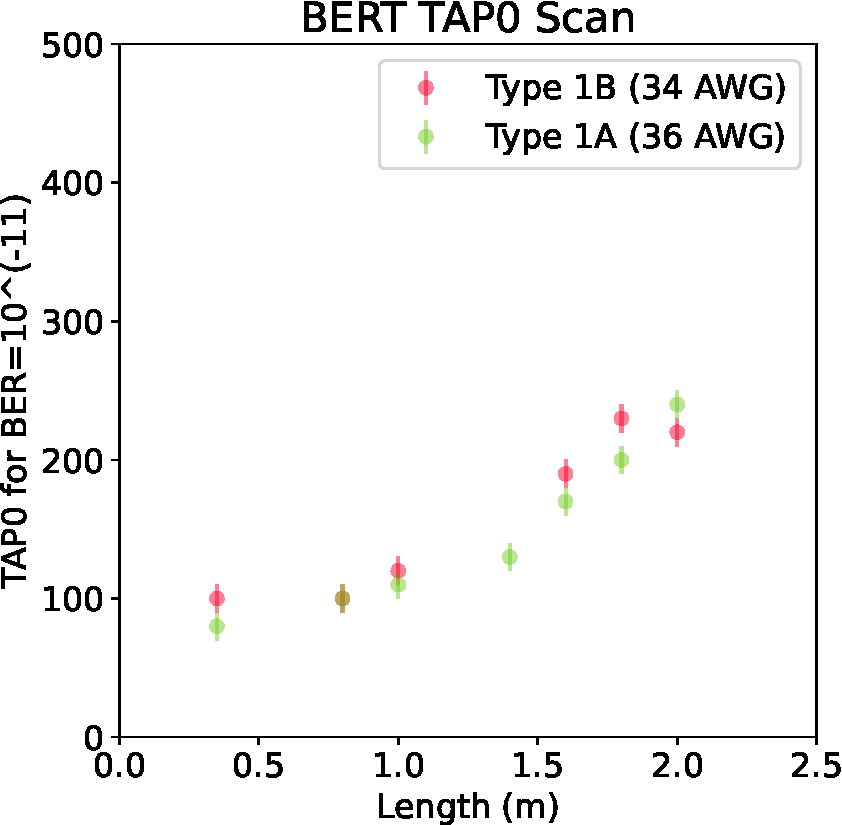
\includegraphics[width=0.40\textwidth,origin=c]{../figures/BERT_TAP0_vs_Length-crop.pdf}
\caption{
\label{fig:tap0_vs_length}
Measurement of signal amplitude (set by TAP0) for electrical links as a function of e-link length for 34 and 36 AWG e-links.
In the hardware setup (left), an FC7 mezzanine card is connected to an SCC through two commercial display port cables, an adapter board, and an e-link for control and readout of an RD53 chip.
The measurements (right) show the TAP0 setting to achieve a bit error rate of $10^{-11}$ for e-links of different lengths and gauges.
}
\end{figure}

% Crosstalk measurements

Furthermore, an external crosstalk measurement was performed, and the results are shown in \fig~\ref{fig:external_crosstalk}.
To mitigate the effect of external crosstalk from a large aggressor amplitude, the victim amplitude set by TAP0 only requires a small increase.
Thus, external crosstalk from the single aggressor e-link has a small effect on readout over the victim e-link.

% use raisebox to adjust vertical spacing
\begin{figure}[htbp]
\centering
\raisebox{-0.4\height}{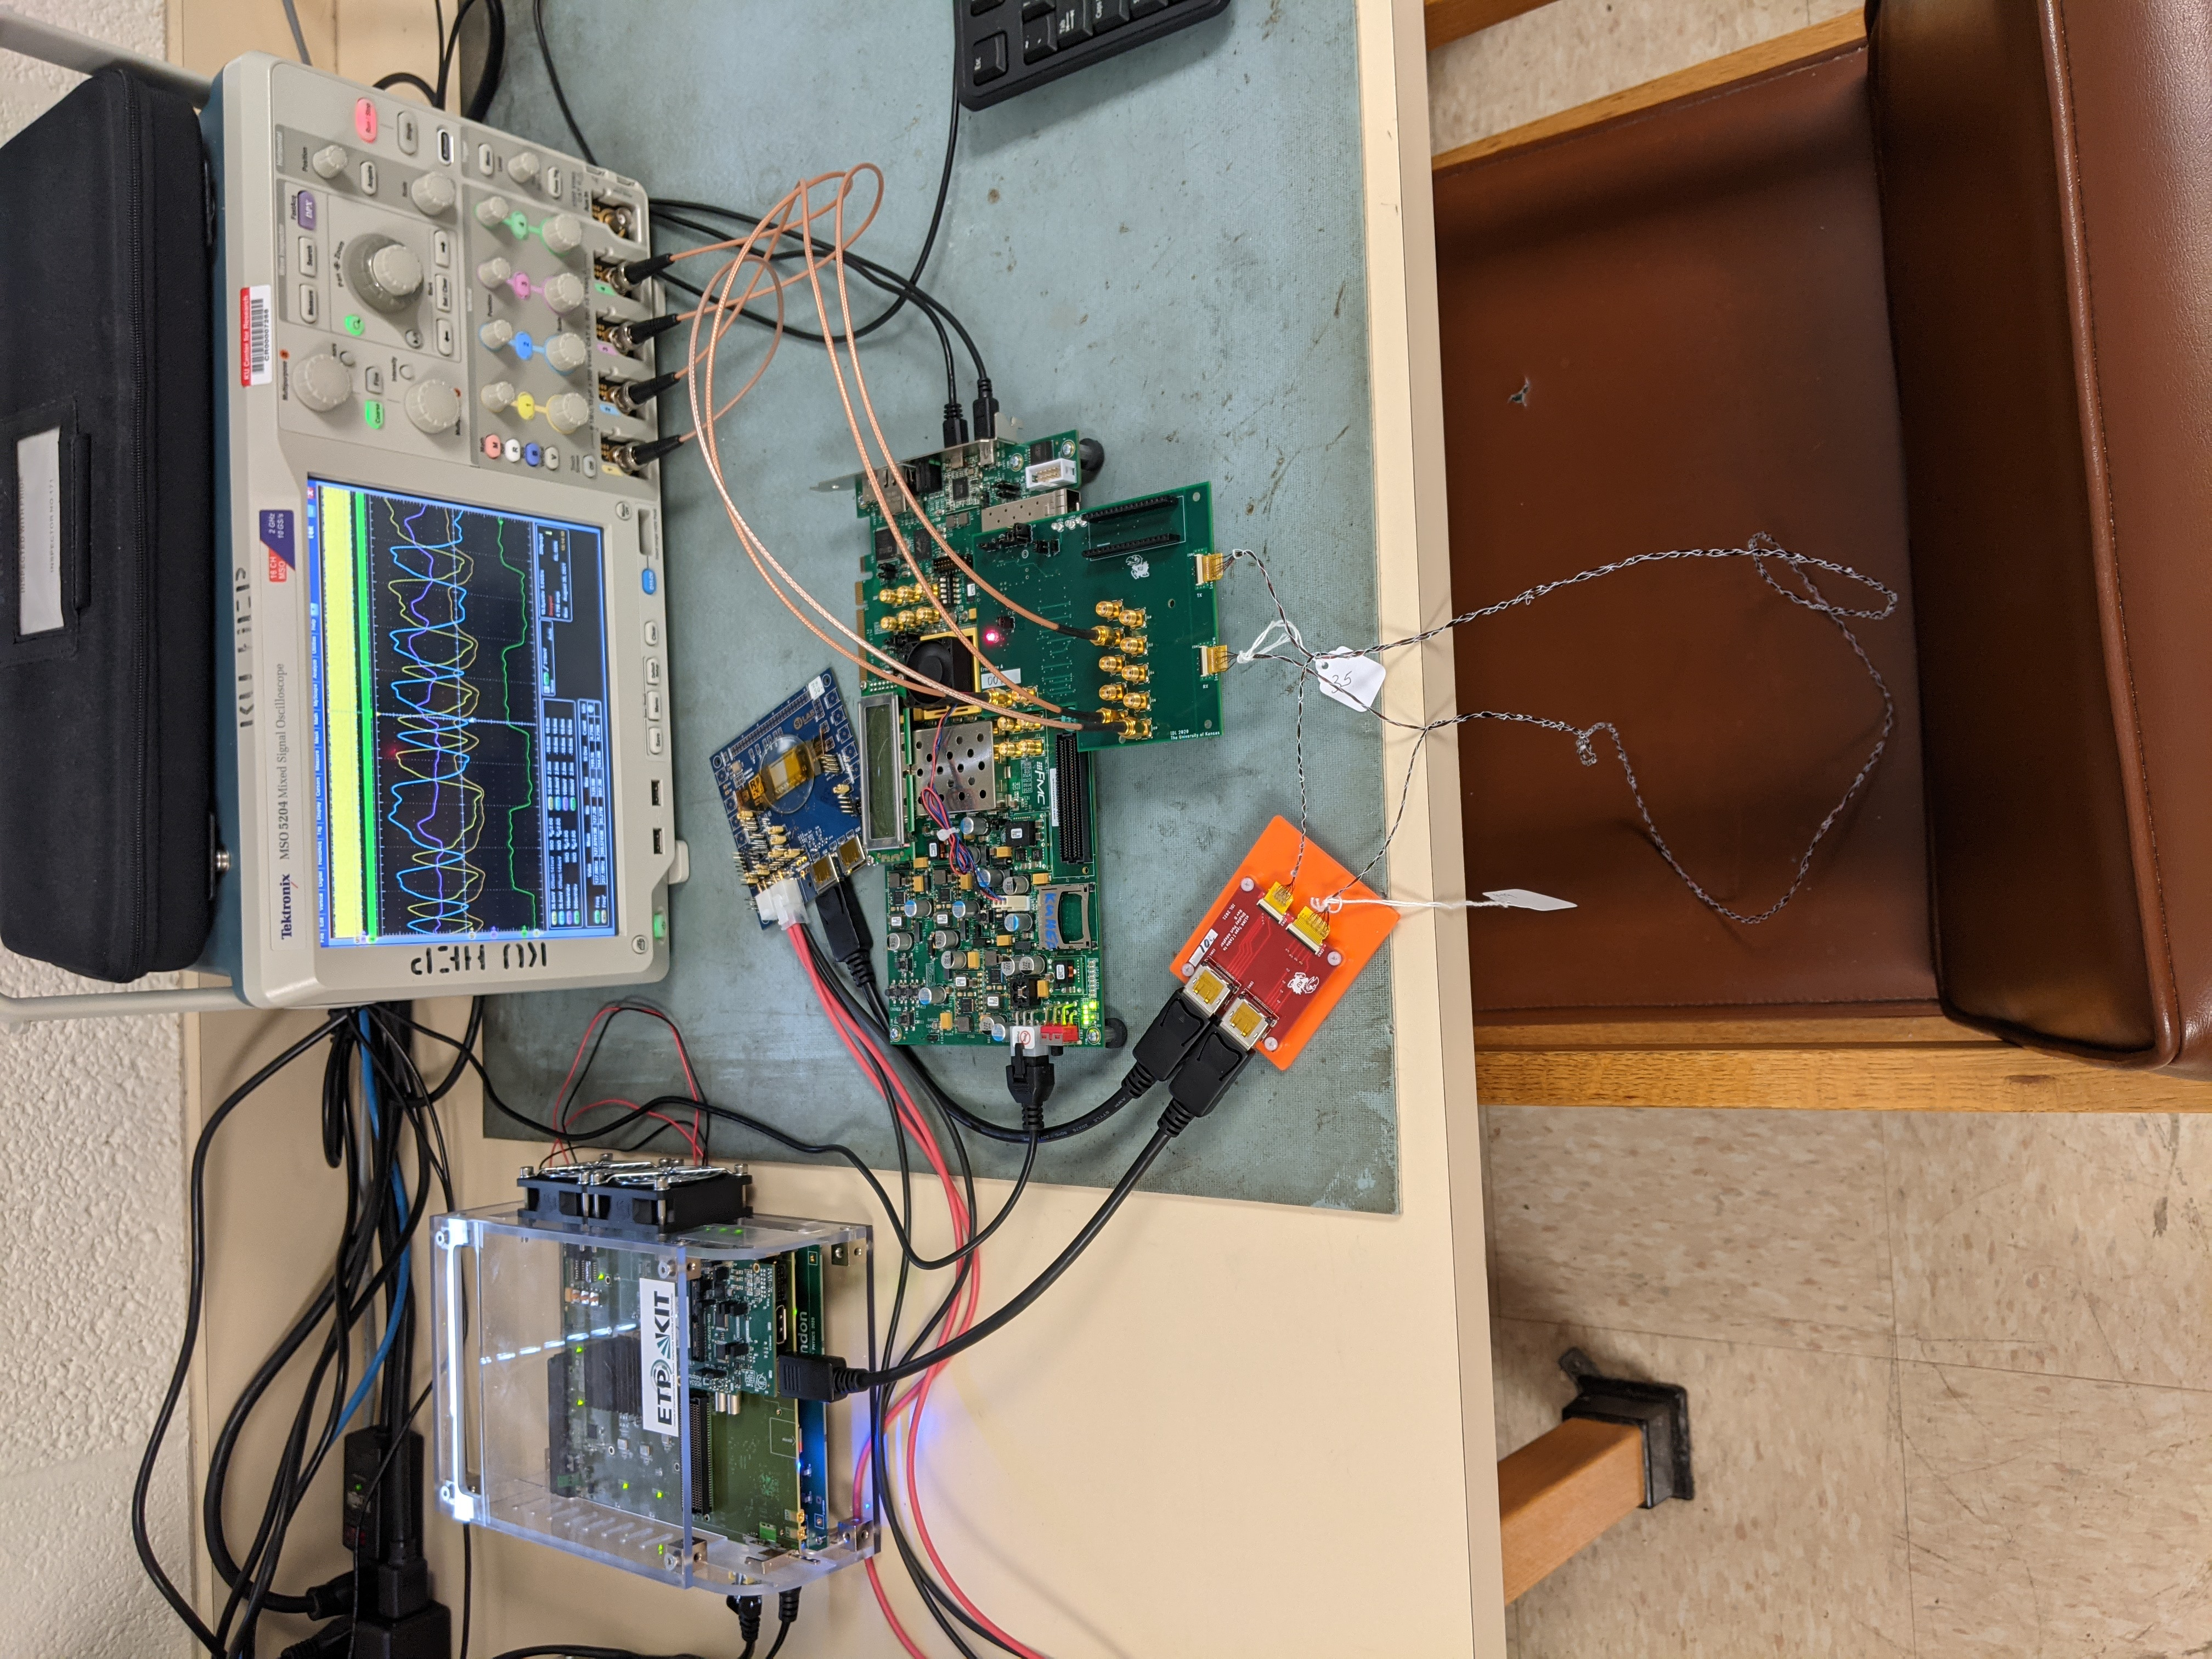
\includegraphics[height=2.0in,origin=c,angle=270]{../figures/external_crosstalk_setup.jpg}}
\hspace*{.2in}
\raisebox{-0.5\height}{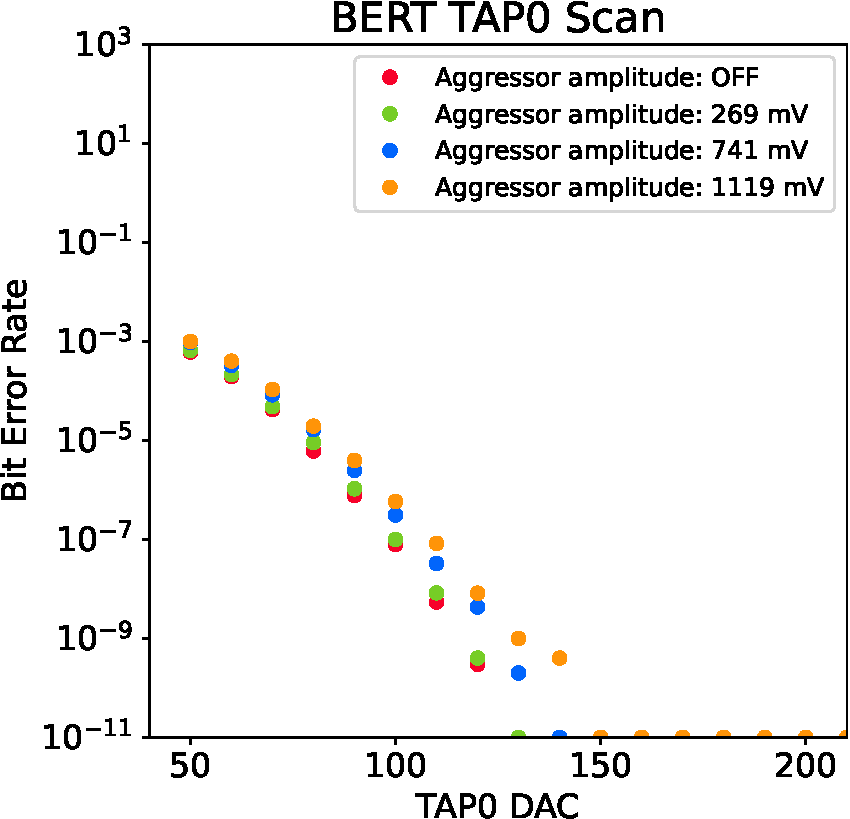
\includegraphics[height=2.75in,origin=c]{../figures/BERT_TAP0_Scan_External_Crosstalk-crop.pdf}}
\caption{
\label{fig:external_crosstalk}
Measurement of the effect of external crosstalk on data transmission.
Two e-links (1.4 meters, 36 AWG) are twisted together (left), with a victim e-link connected between an FC7 mezzanine card and SCC to read from an RD53 chip, and an aggressor e-link connected to a KC705.
The KC705 sends PRBS signals on four e-link channels on the aggressor at different amplitudes.
}
\end{figure}

Radiation testing was performed to determine if e-links can maintain performance after receiving up to 1500 \mrad, which surpasses the total dose expected during their use in CMS.
Two different epoxies, Araldite 2011~(Ref.~\cite{ref:araldite}) and UR6060~(Ref.~\cite{ref:ur}), were used for e-links that underwent radiation testing.
For doses up to 1300 \mrad, the Araldite 2011 epoxy showed significant darkening, while the UR6060 epoxy remained clear and transparent.
The signal integrity on e-links remained good after radiation doses, and UR6060 is chosen as the epoxy used for e-link production.
The polyimide braiding used for lashing becomes brittle after 1900 \mrad, but this should not effect the electrical readout.

\section{Portcards with Optical Links}
\label{sec:optical}

The portcards play an important role in the readout chain in converting electrical signals from on-detector readout chips to optical signals for off-detector DTC boards.
% The portcard design and a photo of a prototype portcard are shown in \fig~\ref{fig:port_card}.
Dedicated setups with the portcards reading out SCCs with short coaxial cables have been used to test the prototype portcard and validate the optical part of the readout chain.
% The optical links have been characterized by various measurements.
In one measurement of the optical links, the high-speed input to the lpGBT is compared to a 5-bit adjustable constant voltage by a comparator sampled with a phase interpolated clock.
Transitions of the comparator are counted; within the eye the output should toggle, but above or below the eye, no transitions are expected.
The data from this measurement are shown in \fig~\ref{fig:lpgbt_eye}.
The high toggle count region is large, corresponding to a large eye diagram and a strong optical signal.

% port card figure
%
% \begin{figure}[htbp]
% \centering
% \raisebox{-0.5\height}{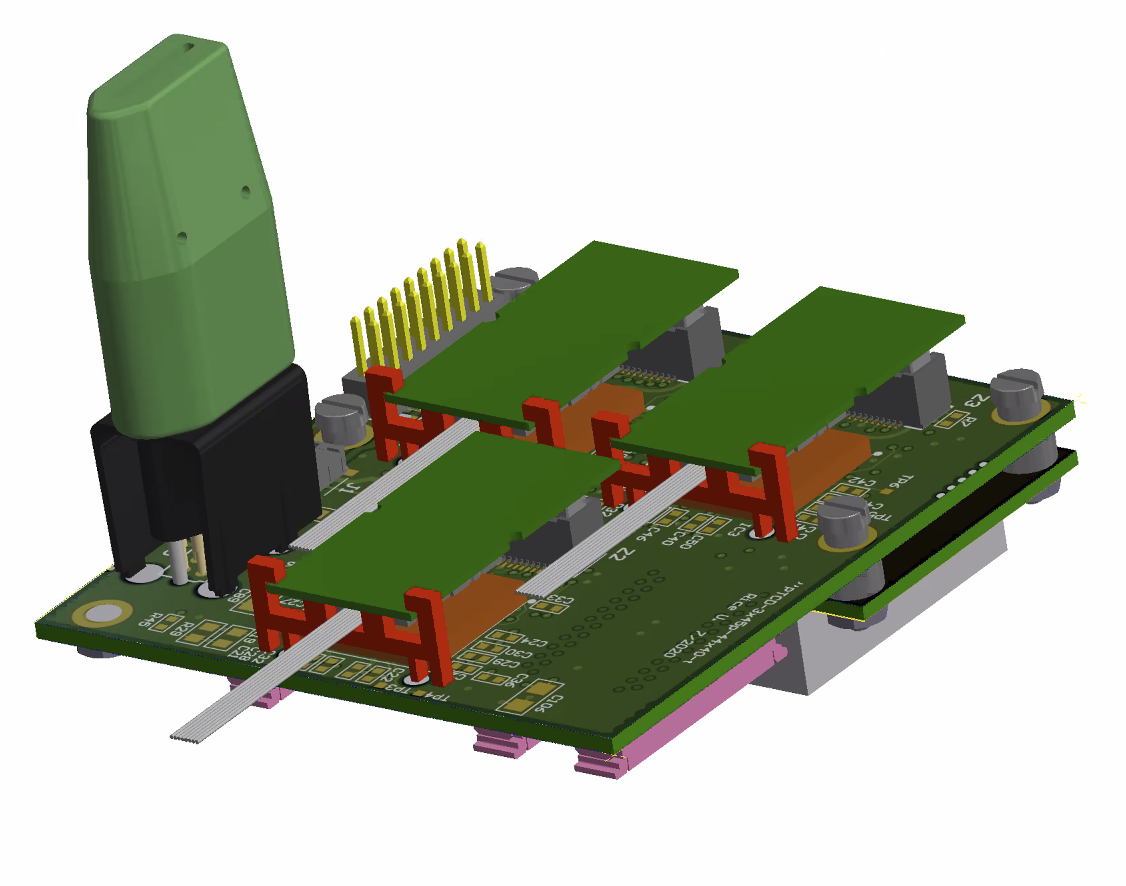
\includegraphics[width=0.30\textwidth,origin=c]{../figures/port_card_design.png}}
% \qquad
% \raisebox{-0.5\height}{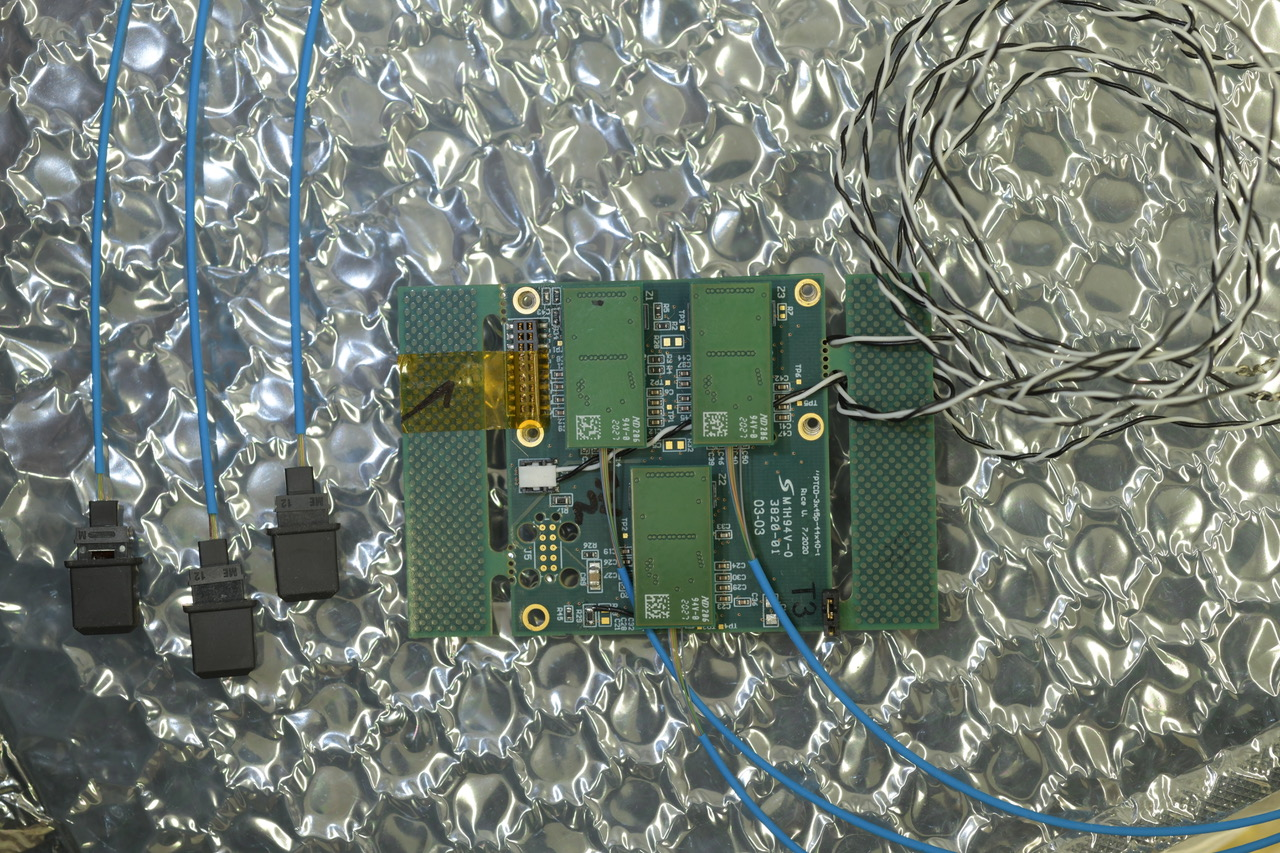
\includegraphics[width=0.30\textwidth,origin=c]{../figures/port_card_back.jpeg}}
% \caption{
% \label{fig:port_card}
% Portcard design (left) and prototype (right).
% The portcard has three lpGBT and three \vtrxp\space modules, which are used to convert high bandwidth electric signals to optical signals.
% }
% \end{figure}

% Optical Link Measurements

\begin{figure}[htbp]
\centering
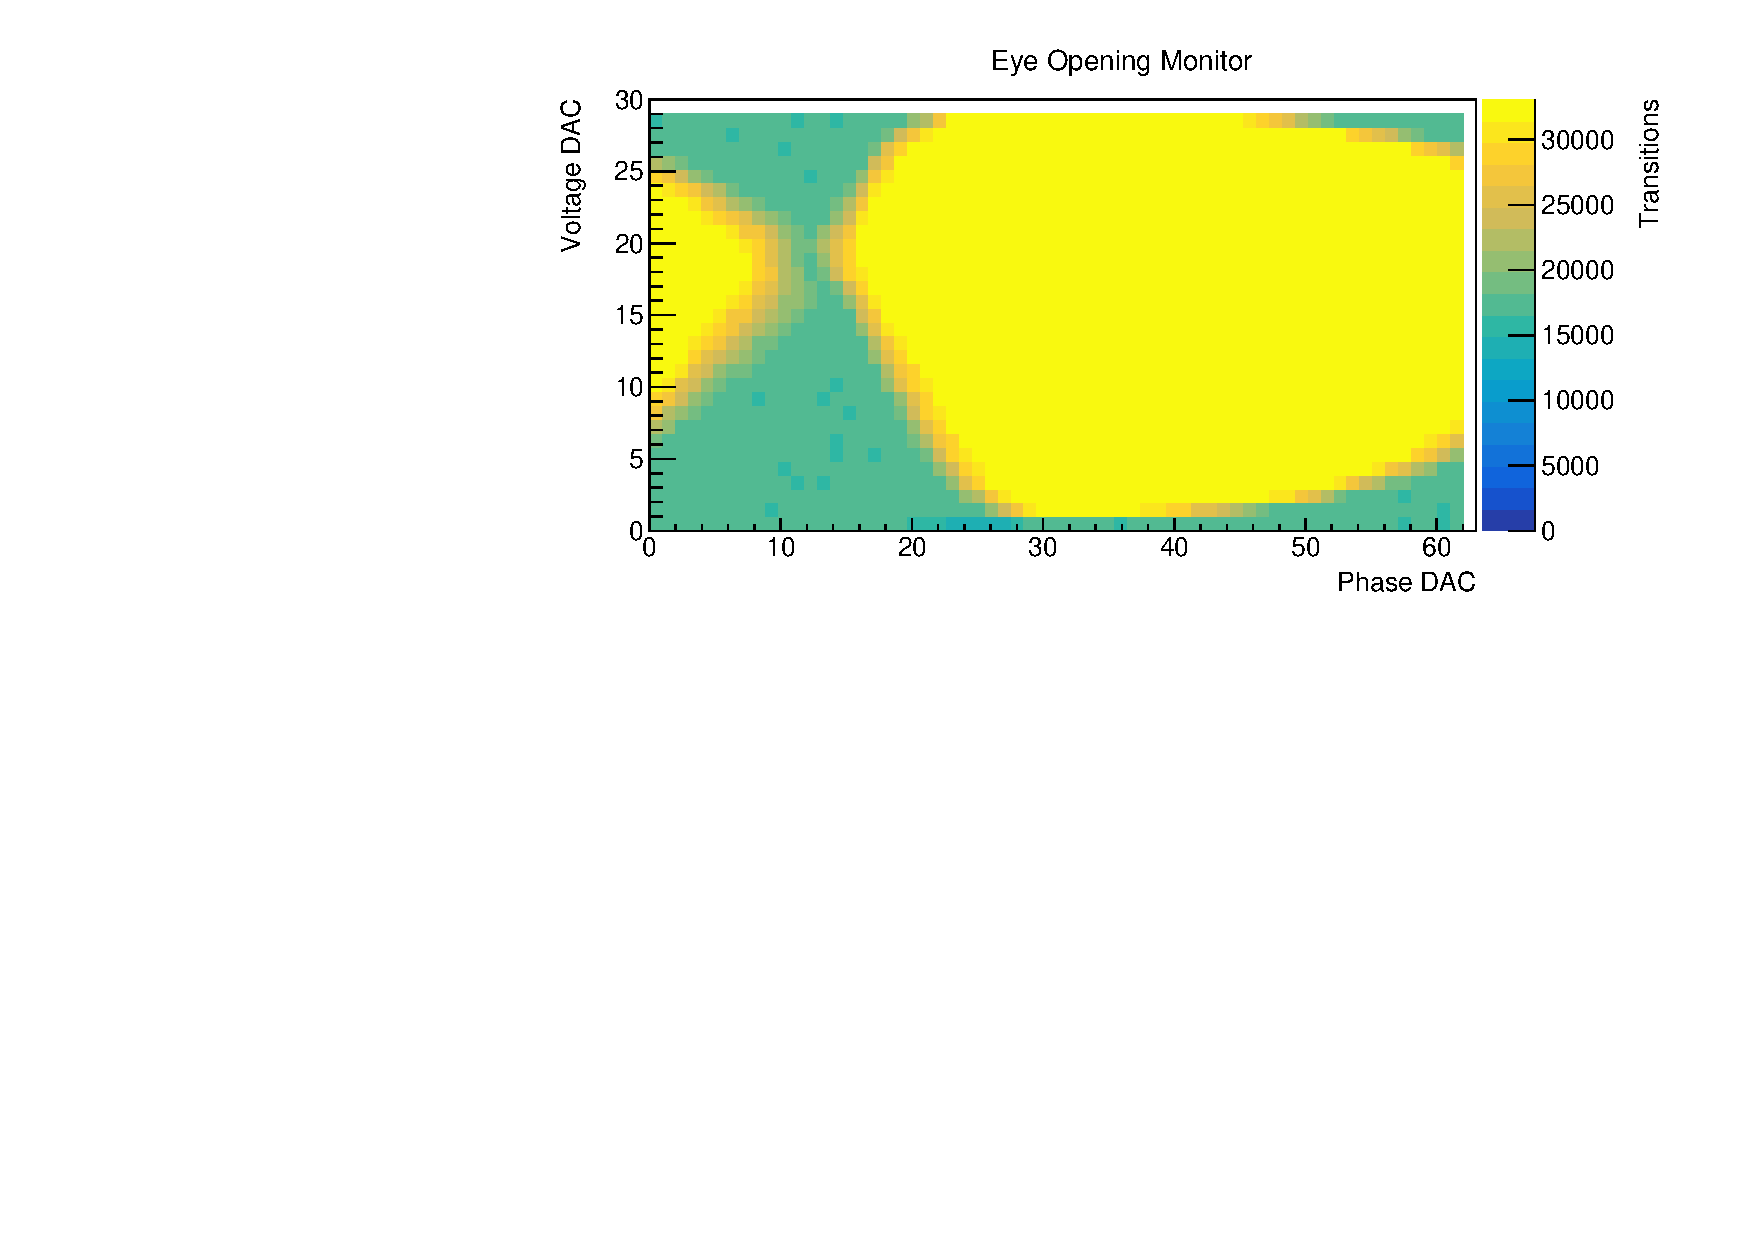
\includegraphics[width=0.70\textwidth,origin=c]{../figures/lpGBT_eye.pdf}
\caption{
\label{fig:lpgbt_eye}
Eye opening monitor from an lpGBT for the 2.56 Gbps optical down link with equalization parameters at default settings.
The vertical axis is a 5-bit encoded DAC value that corresponds to the constant voltage that the high-speed signal is compared with.
The horizontal axis is a 6-bit encoded DAC value that governs the sampling phase used for this comparison.
The color scale shows the number of transitions, which is the toggle count.
Regions with high toggle count correspond to the eye opening, while regions with low toggle count are outside the eye opening.
}
\end{figure}

% Electrical Link Measurements

In addition, the electrical link receivers on the lpGBT are being studied.
In one measurement, the signal source is a PRBS7 generator in the RD53 readout chip.
This signal is sent over a commercial display port cable, an adapter board, and a Molex FPC cable (Ref.~\cite{ref:molex_cable}) to be received by an lpGBT.
The signal is compared to an internal error checker on the lpGBT.
The bit-error rate is measured as a function of clock sampling phase and equalization setting, and the results are provided in \fig~\ref{fig:lpgbt_bert}.
The region with a bit error rate of $9.3 * 10^{-10}$ corresponds to zero errors for the total number of bits checked.
The phases with zero errors are those where the eye diagram is open.
The equalizer on the lpGBT reduces jitter and the bit error rate by processing the high-speed signal to minimize Inter-Symbol-Interferance~\cite{ref:lpgbt_2}.
Changing the equalization setting has only a small effect on the timing.
Low error rates on the lpGBT electrical link receivers are achieved by tuning the sampling phase.

\begin{figure}[htbp]
\centering
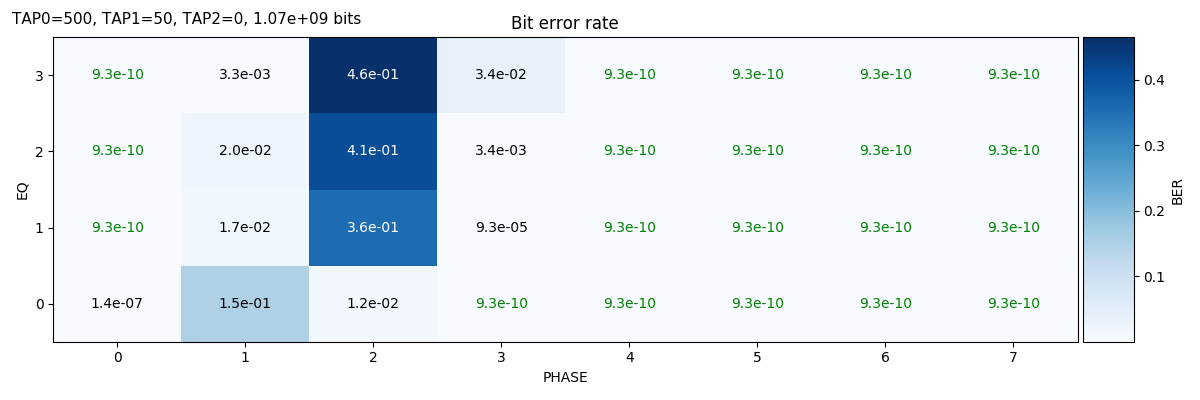
\includegraphics[width=1.0\textwidth,origin=c]{../figures/lpGBT_bert.png}
\caption{
\label{fig:lpgbt_bert}
Scan of bit-error rate vs. clock sampling phase and equalization setting for electrical port receivers on the lpGBT driven by the RD53 pixel readout chip.
The number of bits checked at each setting is $1.07 * 10^{9}$.
Points in green have zero observed errors and report the reciprocal of the number of bits checked.
}
\end{figure}

\section{Conclusion}
\label{sec:conclusion}

% The data readout chain is an important part of the CMS Phase-2 pixel upgrade.
Various system tests have been performed to characterize the electrical and optical links forming the readout chain for the CMS Phase-2 pixel upgrade.
Electrical links can provide stable connectivity at the required lengths, and crosstalk has a small effect on signal quality.
Conversion from electrical to optical links is working well, and the optical links have good performance.
These results form an important input to the final design, production, and testing of components for the pixel detector readout chain.

\acknowledgments

The author would like to thank the National Science Foundation for funding this research.

% We suggest to always provide author, title and journal data:
% in short all the informations that clearly identify a document.

\begin{thebibliography}{99}

% Examples
%
% \bibitem{a}
% Author, \emph{Title}, \emph{J. Abbrev.} {\bf vol} (year) pg.
%
% \bibitem{b}
% Author, \emph{Title},
% arxiv:1234.5678.
%
% \bibitem{c}
% Author, \emph{Title},
% Publisher (year).

% Please avoid comments such as "For a review'', "For some examples",
% "and references therein" or move them in the text. In general,
% please leave only references in the bibliography and move all
% accessory text in footnotes.

% Also, please have only one work for each \bibitem.

% CMS experiment Ref.
% CMS Collaboration, The CMS experiment at the CERN LHC,
% JINST 3 (2008) S08004, doi:10.1088/1748-0221/3/08/S08004

\bibitem{ref:cms}
CMS Collaboration, \emph{The CMS experiment at the CERN LHC},
JINST 3 (2008) S08004.

% HL-LHC Ref.
% @article{Apollinari:2120673,
%       author        = "Apollinari, G. and Brüning, O. and Nakamoto, T. and
%                        Rossi, Lucio",
%       title         = "{Chapter 1: High Luminosity Large Hadron Collider HL-LHC.
%                        High Luminosity Large Hadron Collider HL-LHC}",
%       journal       = "CERN Yellow Report",
%       archivePrefix = "arXiv",
%       eprint        = "1705.08830",
%       reportNumber  = "FERMILAB-PUB-15-699-TD, 5",
%       pages         = "1-19. 21 p",
%       month         = "May",
%       year          = "2017",
%       url           = "https://cds.cern.ch/record/2120673",
%       note          = "21 pages, chapter in High-Luminosity Large Hadron Collider
%                        (HL-LHC) : Preliminary Design Report",
%       doi           = "10.5170/CERN-2015-005.1",
% }

\bibitem{ref:hllhc}
CERN Yellow Report CERN-2015-005, pp.1-19.

% TDR Ref.
%
% @techreport{CERN-LHCC-2017-009,
%       title         = "{The Phase-2 Upgrade of the CMS Tracker}",
%       institution   = "CERN",
%       collaboration = "CMS Collaboration",
%       address       = "Geneva",
%       reportNumber  = "CERN-LHCC-2017-009, CMS-TDR-014",
%       month         = "Jun",
%       year          = "2017",
%       url           = "https://cds.cern.ch/record/2272264",
% }

\bibitem{ref:tdr}
CMS Collaboration, \emph{The Phase-2 Upgrade of the CMS Tracker},
CERN-LHCC-2017-009 (2017).

% S. Orfanelli Ref.
%
% @article{ORFANELLI2020164396,
% 	abstract = {A new silicon tracker will be built for the Phase 2 Upgrade of the CMS experiment to fully exploit the increased luminosity delivered by the HL-LHC. The innermost part, called the Inner Tracker, will be exposed to extreme conditions such as unprecedented radiation levels of 1.2Grad and 2.3×1016 neq/cm2 and hit rate of 3.2GHz/cm2. The new Inner Tracker relies on many novel solutions and technologies that allow for a design of a light and radiation-hard pixel detector of high performance. The hybrid pixel modules will be composed of pixel sensors with pixel size of 2500μm2 and a new ASIC, designed in 65 nm CMOS technology, developed by the RD53 collaboration. A novel scheme of serial powering will be deployed to power the pixel modules and new technologies will be used for a high bandwidth readout system. The mechanics will be lightweight, based on carbon-fibre material and two-phase CO2 cooling. In this contribution, the design of the CMS Inner Tracker system will be presented along with the prospective design choices.},
% 	author = {S. Orfanelli},
% 	doi = {https://doi.org/10.1016/j.nima.2020.164396},
% 	issn = {0168-9002},
% 	journal = {Nuclear Instruments and Methods in Physics Research Section A: Accelerators, Spectrometers, Detectors and Associated Equipment},
% 	keywords = {Silicon detectors, Inner tracker, Readout electronics, Serial powering},
% 	pages = {164396},
% 	title = {The Phase 2 Upgrade of the CMS Inner Tracker},
% 	url = {https://www.sciencedirect.com/science/article/pii/S0168900220307932},
% 	volume = {980},
% 	year = {2020},
% 	Bdsk-Url-1 = {https://www.sciencedirect.com/science/article/pii/S0168900220307932},
% 	Bdsk-Url-2 = {https://doi.org/10.1016/j.nima.2020.164396}
% }

\bibitem{ref:orfanelli}
S. Orfanelli, \emph{The Phase 2 Upgrade of the CMS Inner Tracker},
Nuclear Instruments and Methods in Physics Research Section A: Accelerators, Spectrometers, Detectors and Associated Equipment, Volume 980 (2020).

% RD53 Ref.
%
% @techreport{Garcia-Sciveres:2287593,
%       author        = "Garcia-Sciveres, Maurice",
%       title         = "{The RD53A Integrated Circuit}",
%       institution   = "CERN",
%       collaboration = "RD53 Collaboration",
%       address       = "Geneva",
%       reportNumber  = "CERN-RD53-PUB-17-001",
%       month         = "Oct",
%       year          = "2017",
%       url           = "https://cds.cern.ch/record/2287593",
% }

\bibitem{ref:rd53}
M. Garcia-Sciveres, \emph{The RD53A Integrated Circuit},
CERN-RD53-PUB-17-001 (2017).

% VTRx+ Ref.
%
% @article{So_s_2017,
% 	abstract = {The Versatile Link PLUS project targets the phase II upgrades of the ATLAS and CMS experiments. It will develop a radiation resistant optical link, operating at up to 10 Gb/s in the upstream and up to 5 Gb/s in the downstream directions with a smaller footprint and higher channel count than its predecessor. A low-profile package is being developed that allows volume production at reduced costs, but which nevertheless can be configured to suit the individual channel count needs of different detectors. This paper describes the development strategies and summarizes the status of the feasibility demonstration phase of the project.},
% 	author = {C. So{\'{o}}s and S. D{\'{e}}traz and L. Olanter{\"a} and C. Sigaud and J. Troska and F. Vasey and M. Zeiler},
% 	doi = {10.1088/1748-0221/12/03/c03068},
% 	journal = {Journal of Instrumentation},
% 	month = {mar},
% 	number = {03},
% 	pages = {C03068--C03068},
% 	publisher = {{IOP} Publishing},
% 	title = {Versatile Link {PLUS} transceiver development},
% 	url = {https://doi.org/10.1088/1748-0221/12/03/c03068},
% 	volume = {12},
% 	year = 2017,
% 	Bdsk-Url-1 = {https://doi.org/10.1088/1748-0221/12/03/c03068}
% }

\bibitem{ref:vtrxp}
C. So{\'{o}}s, et al., \emph{Versatile Link {PLUS} transceiver development},
Proceedings on the Topical Workshop on Electronics for Particle Physics, TWEPP 2016,
Journal of Instrumentation (2017).

% lpGBT Ref.
% https://indico.cern.ch/event/799025/contributions/3486153/
% Title: The lpGBT: a radiation tolerant ASIC for Data, Timing, Trigger and Control Applications in HL-LHC
% Author: Paulo Moreira
% Conference: TWEPP
% Year: 2019

\bibitem{ref:lpgbt_1}
P. Moreira, et al., \emph{The lpGBT: A radiation tolerant ASIC for Data, Timing, Trigger and Control Applications in HL-LHC},
Proceedings on the Topical Workshop on Electronics for Particle Physics, TWEPP 2019.

% lpGBT documentation
% https://twiki.nevis.columbia.edu/twiki/pub/ATLAS/SliceTestboard/lpGBT.pdf

\bibitem{ref:lpgbt_2}
\url{https://twiki.nevis.columbia.edu/twiki/pub/ATLAS/SliceTestboard/lpGBT.pdf}.

% Araldite 2011 is from the Huntsman Corporation.
% https://www.huntsman.com/products/araldite2000/araldite-2011

\bibitem{ref:araldite}
\url{https://www.huntsman.com/products/araldite2000/araldite-2011}.

% UR6060 is a product of Resinlab, and we purchase it from https://www.ellsworth.com/.
% https://www.ellsworth.com/products/encapsulants/polyurethane/resinlab-ur6060-polyurethane-encapsulant-clear-50-ml-cartridge/

\bibitem{ref:ur}
\url{https://www.ellsworth.com/products/encapsulants/polyurethane/resinlab-ur6060-polyurethane-encapsulant-clear-50-ml-cartridge}.

% FC7 mezzanine card
\bibitem{ref:fc7}
\url{https://espace.cern.ch/project-FC7/SitePages/Home.aspx}.

% Molex connectors
%
% The company name is Molex.
% https://www.molex.com/molex/home
%
% 17 position part number is 5025981793
% https://www.molex.com/molex/products/part-detail/ffc_fpc_connectors/5025981793
%
% 33 position part number is 5025983393
% https://www.molex.com/molex/products/part-detail/ffc_fpc_connectors/5025983393
%
% 45 position part number is 5025984593
% https://www.molex.com/molex/products/part-detail/ffc_fpc_connectors/5025984593

% \bibitem{ref:molex17}
% \url{https://www.molex.com/molex/products/part-detail/ffc_fpc_connectors/5025981793}.

% \bibitem{ref:molex33}
% \url{https://www.molex.com/molex/products/part-detail/ffc_fpc_connectors/5025983393}.

\bibitem{ref:molex45}
\url{https://www.molex.com/molex/products/part-detail/ffc_fpc_connectors/5025984593}.

\bibitem{ref:molex_cable}
\url{https://www.molex.com/molex/products/family/premoflex?parentKey=ffc_fpc_connectors}.

\end{thebibliography}
\end{document}
